\documentclass{article}

\usepackage[margin=1in]{geometry}

\usepackage{graphicx}
\graphicspath{{Document-images/}}


\title{Requirements Specification: Dungeons \& Dragons 5E Character Tools}
\author{Christopher Evans - https://github.com/cevans88}

\begin{document}

\maketitle

\section{Introduction}

This document is the Software Requirements Specification document for the Dungeons \& Dragons 5th Edition Character Tools application . It will serve to unambiguously define the requirements of the application so that efforts in later stages of the development cycle may be more focused and effective.


\subsection{Purpose}

By formally defining the requirements of the application this document benefits the project in a number of ways:

\begin{description}
	\item [Reduces the development effort.] Explicitly specifying the requirements at the outset of the project minimises the amount of redesign, recording, and retesting. It can also expose omissions and inconsistencies earlier in the development cycle where such problems require less effort to rectify.
	\item [Provides a basis for validation.] Design and implementation compliance plans can be produced using this SRS as a reference.
\end{description}\\
It is divided into \textbf{X} parts:

The intended audience for this document includes the design, development, and testing teams who will find its contents invaluable as a basis for their work (whether that be designing interfaces or writing test suites to verify the meeting of specific requirements).


\subsection{Scope}

Application: Dungeons \& Dragons 5th Edition Character Tools

The intent of the application is to provide desktop GUI tools for creating, viewing, and storing characters in the D\&D 5E ruleset. Users will be able to make selections from the various player classes, backgrounds, races, and equipment lists, as well as customise the statistics, equipment, and levels of characters once they have been created.

By consolidating all the choices that are found across the various books and supplements available to players into one application and providing a means of easily creating and viewing characters with those choices the application aims to streamline the process of planning or experimenting with characters.

Additional features which the application could be extended with include a combat simulation facility, the option of sharing or exporting character profiles with others, and implementing the suite as a web application.

In order to provide an effective character creation suite it will be necessary for the application to:

- Accurately model the systems present in D\&D 5E;
- Be up to date on all the available character options that exist across the D\&D 5E books;
	- Since additional releases are inevitable the application should be able to easily integrate further options.
- Provide a GUI that:
	- Is pleasing to the eye;
	- Presents all the desired character information in a useful way, that is:
		- Can all be viewed at once if needed;
		- Can be contrasted with other options;
		- Is self-explanatory either through labels or tooltips.
	- Makes it easy to make selections or edits.

In order to provide a combat simulation facility the application will need to be extended to include:

- Data for modelling the various creatures that can be involved in combat with player characters;
- Accurate modelling of the combat systems in D\&D5E;
- A suitable interface for setting up, running, and analysing combat encounters.
- Since D\&D5E combat is often represented as a grid of 5" by 5" squares it would make sense to base the interface around this model;
- The scope of this feature does not extend to implementing an artificial intelligence system for creatures in the combat scenario.

Enabling the sharing or exporting of character profiles will require the application to be able to convert the totality of a character's attributes to a string, and in turn be able to import such a string and construct the same character entity.

Implementing the suite as a web application would entail embedding it into a website so that users will not have to run an executable on their desktop computer to use the application.



\subsection{References}
% This subsection should:
% - Provide a complete list of documents referenced elsewhere in the SRS;
% - Identify each document by title, report number (if applicable), date, and publishing organisation;
% - Specify the sources from which the references can be obtained.

% This information may be provided by reference to an appendix or to another document.


This SRS shall be used in conjunction with the following documents:

D\&D5E Character Sheet, \ref{fig:appa}, Wizards of the Coast LLC, 28/08/2017.

D\&D5E Spellcasting Sheet, \ref{fig:appb}, Wizards of the Coast LLC, 28/08/2017.


\subsection{Definitions, acronyms, and abbreviations}
% This subsection should provide the definitions of all terms, acronyms, and abbreviations required to properly interpret the SRS. This information may be provided by reference to one or more appendixes in the SRS or by reference to other documents.

In order to fully disambiguate terms used in this SRS a number of key terms are defined below:

\subsubsection{Dungeons \& Dragons 5th Edition:}
The 5th edition rules system for the Dungeons \& Dragons roleplaying game made and owned by Wizards of the Coast LLC. Since the rules and mechanics vary between different editions of the game it is important to define which edition the application is intended to model. The rules and mechanics being modelled are found in the 5th Edition Player's Handbook, errata clarification documents, and the wide range of supplement material that is produced for players such as the 5th Edition Sword Coast Adventurer's Guide.

\subsubsection{D\&D5E:}
Acronym for Dungeon's \& Dragons 5th Edition. "5E" also used in isolation to abbreviate "5th Edition".


\subsubsection{Character:}
A character in the context of D\&D5E is an entity comprised of many different attributes that have been selected from a variety of options by a player including, but not limited to:

- Name (e.g. Tiberius)
- Race (e.g. Dwarf)
- Class (e.g. Fighter)
- Background (e.g. Folk Hero)

A comprehensive picture of the elements that make up a character can be seen by examining the D\&D5E Character Sheet(MAKE A HYPERLINK) included in the Appendix.

\subsubsection{Player}
The person making a D\&D5E character, synonymous with "user" of the D\&D5E Character Tools application.



\subsection{Overview}
% This subsection should:
% - Describe what the rest of the SRS contains;
% - Explain how the SRS is organised.






\section{Overall description}
% This section of the SRS should describe the general factors that affect the product and its requirements. This section does not state specific requirements. Instead, it provides a background for those requirements, which are defined in detail in the Specific Requirements section later. Instead, it provides a background for those requirements, which are defined in detail in Section 3 of the SRS, and makes them easier to understand.
% This section usually consists of six subsections as follows:
% - Product perspective;
% - Product functions;
% - User characteristics;
% - Constraints;
% - Assumptions and dependencies;
% - Apportioning of requirements.

\subsection{Product perspective}
% This subsection of the SRS should put the product into perspective with other related products. If the product is independent and totally self-contained, it should be so stated here. If the SRS defines a product that is a component of a larger system, as frequently occurs, then this subsection should relate the requirements of that larger system to functionality of the software and should identify interfaces between that system and the software.

% A block diagram showing the major components of the larger system, interconnections, and external interfaces can be helpful.

% This subsection should also describe how the software operates inside various constraints. For example, these constraints could include:
% - System interfaces;
% - User interfaces;
% - Hardware interfaces;
% - Software interfaces;
% - Communications interfaces;
% - Memory;
% - Operations;
% - Site adaptation requirements.

\subsubsection{System interfaces}
% This should list each system interface and identify the functionality of the software to accomplish the system requirement and the interface description to match the system.

\subsubsection{User interfaces}
% This should specify the following:
% - The logical characteristics of each interface between the software product and its users. This includes those configuration characteristics (e.g. required screen formats, page or window layouts, content of any reports or menus, or availability of programmable function keys) necessary to accomplish the software requirements.
% - All the aspects of optimising the interface with the person who must use the system. This may simply comprise a list of do's and dont's on how the system will appear to the user. One example may be a requirement for the option of long or short error messages. Like all others, these requirements should be verifiable, e.g. "a clerk typist grade 4 can do function X in Z min after 1 h of training" rather than "a typist can do function X." (This may also be specified in the Software System Attributes under a section titled Ease of Use.)

\subsubsection{Hardware interfaces}
% This should specify the logical characteristics of each interface between the software product and the hardware components of the system. This includes configuration characteristics (number of ports, instruction sets, etc.). It also covers such matters as what devices are to be supported, how they are to be supported, and protocols. For example, terminal support may specify full-screen support as opposed to line-by-line support.


\subsubsection{Software interfaces}
% This should specify the use of other required software products (e.g., a data management system, an operating system, or a mathematical package), and interfaces with other application systems (e.g. the linkage between an accounts receivable system and a general ledger system). For each required software product, the following should be provided:
% - Name;
% - Mnemonic;
% - Specification number;
% - Version number;
% - Source.

% For each interface, the following should be provided:
% - Discussion of the purpose of the interfacing software as related to this software product;
% - Definition of the interface in terms of message content and format. It is not necessary to detail any well-documented interface, but a reference to the document defining the interface is required.

\subsubsection{Communications interfaces}
% This should specify the various interfaces to communications such as local network protocols, etc.

\subsubsection{Memory constraints}
% This should specify any applicable characteristics and limits on primary and secondary memory.

\subsubsection{Operations}
% This should specify the normal and special operations required by the user such as:
% - The various modes of operations in the user organisation (e.g. user-initiated operations);
% - Periods of interactive operations and periods of unattended operations;
% - Data processing support functions;
%- Backup and recovery operations.

% NOTE - This is sometimes specified as part of the User Interfaces sections.


\subsubsection{Site adaptation requirements}
% This should:
% - Define the requirements for any data or initialisation sequences that are specific to a given site, mission, or operational mode (e.g., grid values, safety limits, etc.);
% - Specify the site or mission-related features that should be modified to adapt the software to a particular installation.



\subsection{Product functions}
% This subsection of the SRS should provide a summary of the major functions that the software will perform. For example, an SRS for an accounting program may use this part to address customer account maintenance, customer statement, and invoice preparation without mentioning the vast amount of detail that each of those functions requires.

% Sometimes the function summary that is necessary for this part can be taken directly from the section of the higher-level specification (if one exists) that allocates particular functions to the software product. Note that for the sake of clarity:
% - The functions should be organised in a way that makes the list of functions understandable to the customer or to anyone else reading the document for the first time.
% - textual or graphical models can be used to show the different functions and their relationships. Such a diagram is not intended to show a design of a product, but simply shows the logical relationships among variables.


\subsection{User characteristics}
% This subsection of the SRS should describe those general characteristics of the intended users of the product including educational level, experience, and technical expertise. It should not be used to state specific requirements, but rather should provide the reasons why certain specific requirements are later specified in Section 3 of the SRS.


\subsection{Constraints}
% This subsection of the SRS should provide a general description of any other items that will limit the developer's options. These include:
% - Regulatory policies;
% - Hardware limitations (e.g. signal timing requirements);
% - Interfaces to other applications;
% - Parallel operation;
% - Audit functions;
% - Control functions;
% - Higher-order language requirements;
% - Signal handshake protocols (e.g. XON-XOFF, ACK-NACK);
% - Reliability requirements;
% - Criticality of the application;
% - Safety and security considerations.

\subsection{Assumptions and dependencies}
% This subsection of the SRS should list each of the factors that affect the requirements stated in the SRS. These factors are not design constraints on the software but are, rather, any changes to them that can affect the requirements in the SRS. For example, an assumption may be that a specific operating system will be available on the hardware designated for the software product. If, in fact, the operating system is not available, the SRS would then have to change accordingly.


\subsection{Apportioning of requirements}
% This subsection of the SRS should identify requirements that may be delayed until future versions of the system.



\section{Specific requirements}
% This section of the SRS should contain all of the software requirements to a level of detail sufficient to enable designers to design a system to satisfy those requirements, and testers to test that the system satisfies those requirements. Throughout this section, every stated requirement should be externally perceivable by users, operators, or other external systems. These requirements should include at a minimum a description of every input (stimulus) into the system, every output (response) from the system, and all functions performed by the system in response to an input or in support of an output. As this is often the largest and most important part of the SRS, the following principles apply:
% - Specific requirements should be stated in conformance with all the characteristics described in 4.3a.
% - Specific requirements should be cross-referenced to earlier documents that relate.
% - All requirements should be uniquely identifiable.
% - Careful attention should be given to organising the requirements to maximise readability.

% Before examining specific ways of organising the requirements it is helpful to understand the various items that comprise requirements as describe in the following sub-sections.


\subsection{External interfaces}
% This should be a detailed description of all inputs into and outputs from the software system. It should complement the interface descriptions in 5.2 and should not repeat information there.

% It should include both content and format as follows:
% - Name of item;
% - Description of purpose;
% - Source of input or destination of output;
% - Valid range, accuracy, and/or tolerance;
% - Units of measure;
% - Timing;
% - Relationships to other inputs/outputs;
% - Screen formats/organisation;
% - Window formats/organisation;
% - Data formats;
% - Command formats;
% - End messages.

\subsection{Functions}
% Functional requirements should define the fundamental actions that must take place in the software in accepting and processing the inputs and in processing and generating the outputs. These are generally listed as "shall" statements starting with "The system shall..."

% These include:
% - Validity checks on the inputs;
% - Exact sequence of operations;
% - Responses to abnormal situations, including:
	% - Overflow;
	% - Communication and facilities;
	% - Error handling and recovery.
% - Effect of parameters;
% - Relationship of outputs to inputs, including:
	% - Input/output sequences;
	% - Formulas for input to output conversions.

% It may be appropriate to partition the functional requirements into subfunctions or subprocesses. This does not imply that the software design will also be partitioned this way.

\subsection{Performance requirements}
% This subsection should specify both the static and the dynamic numerical requirements placed on the software or on human interaction with the software as a whole. Static numerical requirements may include the following:
% - The number of terminals to be supported;
% - The number of simultaneous users to be supported;
% - Amount and type of information to be handled.

% Static numerical requirements are sometimes identified under a separate section entitled Capacity.

% Dynamic numerical requirements may include, for example, the numbers of transactions and tasks and the amount of data to be processed within certain time periods for both normal and peak workload conditions.

% All of these requirements should be stated in measurable terms.

% For example:
	% '95% of the transactions shall be processed in less than 1 s.'
% Rather than:
	% 'An operator shall not have to wait for the transaction to complete.'

% NOTE - Numerical limits applied to one specific function are normally specified as part of the processing subparagraph.


\subsection{Logical database requirements}
% This should specify the logical requirements for any information that is to be placed into a database. This may include the following:
% - Types of information used by various functions;
% - Frequency of use;
% - Accessing capabilities;
% - Data entities and their relationships;
% - Integrity constraints;
% - Data retention requirements.


\subsection{Design constraints}
% This should specify design constraints that can be imposed by other standards, hardware limitations, etc.

\subsubsection{Standards compliance}
% This subsection should specify the requirements derived from existing standards or regulations. They may include the following:
% - Report format;
% - Data naming;
% - Accounting procedures;
% - Audit tracing.

% For example, this could specify the requirement for software to trace processing activity. Such traces are needed for some applications to meet minimum regulatory or financial standards. An audit trace requirement may, for example, state that all changes to a payroll database must be recorded in a trace file with before and after values.


\subsection{Software system attributes}
% There are a number of attributes of software that can serve as requirements. It is important that required attributes be specified so that their achievement can be objectively verified. A partial list of examples is provided below.

\subsubsection{Reliability}
% This should specify the factors required to establish the required reliability of the software system at time of delivery.

\subsubsection{Availability}
% This should specify the factors required to guarantee a defined availability level for the entire system such as checkpoint, recovery, and restart.

\subsubsection{Security}
% This should specify the factors that protect the software from accidental or malicious access, use, modification, destruction, or disclosure. Specific requirements in this area could include the need to:
% - Utilise certain cryptographical techniques;
% - Keep specific log or history data sets;
% - Assign certain functions to different modules;
% - Restrict communications between some areas of the program;
% - Check data integrity for critical variables.

\subsubsection{Maintainability}
% This should specify attributes of software that relate to the ease of maintenance of the software itself. There may be some requirement for certain modularity, interfaces, complexity, etc. Requirements should not be placed here just because they are thought to be good design practices.


\subsubsection{Portability}
% This should specify attributes of software that relate to the ease of porting the software to other host machines and/or operating systems. This may include the following:
% - Percentage of components with host-dependent code;
% - Percentage of code that is host dependent;
% - Use of a proven portable language;
% - Use of a particular compiler or language subset;
% - Use of a particular operating system.


\subsection{Organising the specific requirements}
% For anything but trivial systems the detailed requirements tend to be extensive. For this reason, it is recommended that careful consideration be given to organising these in a manner optimal for understanding. There is no one optimal organisation for all systems. Different classes of systems lend themselves to different organisations of requirements in Section 3 of the SRS. Examples of some of these organisations are described below:

\subsubsection{System mode}
% Some systems behave quite differently depending on the mode of operation. For example, a control system may have different sets of functions depending on its mode: training, normal, or emergency. When organising this section by mode, the outline A.1 or A.2 should be used. The choice depends on whether interfaces and performance and dependent on mode.

\subsubsection{User class}
% Some systems provide different sets of functions to different classes of users. For example, an elevator control system presents different capabilities to passenger, maintenance workers, and fire fighters. When organising this section by user class, the outline in A.3 should be used.

\subsubsection{Objects}
% Objects are real-world entities that have a counterpart within the system. For example, in a patient monitoring system, objects include patients, sensors, nurses, rooms, physicians, medicines, etc. Associated with each object is a set of attributes (of that object) and functions (performed by that object). These functions are also called services, methods, or processes. When organising this section by object, the outline in A.4 should be used. Note that sets of objects may share attributes and services. These are grouped together as classes.

\subsubsection{Feature}
% A feature is an externally desired service by the system that may require a sequence of inputs to effect the desired result. For example, in a telephone system, features include local call, call forwarding, and conference call. Each feature is generally described in a sequence of stimulus-response pairs. When organising this section by feature, the outline in A.5 should be used.

\subsubsection{Stimulus}
% Some systems can be best organised by describing their functions in terms of stimuli. For example, the functions of an automatic aircraft landing system may be organised into sections for loss of power, wind shear, sudden change in roll, vertical velocity excessive, etc. When organising this section by stimulus, the outline in A.6 should be used.

\subsubsection{Response}
% Some systems can be best organised by describing all the functions in support of the generation of a response. For example, the functions of a personnel system may be organised into sections corresponding to all functions associated with generating paychecks, all functions associated with generating a current list of employees, etc. The outline in A.6 (with all occurrences of stimulus replaced with response should be used.

\subsubsection{Functional hierarchy}
% When none of the above organisational schemes prove helpful, the overall functionality can be organised into a hierarchy of functions organised by either common inputs, common outputs, or common internal data access. Data flow diagrams and data dictionaries can be used to show the relationships between and among the functions and data. When organising this section by functional hierarchy, the outline in A.7 should be used.


\subsection{Additional comments}
% Whenever a new SRS is contemplated, more than one of the organisational techniques previously outlined may be appropriate. In such cases, organise the specific requirements for multiple hierarchies tailored to the specific needs of the system under specification. For example, see A.8 for an combining user and class and feature. Any additional requirements may be put in a separate section at the end of the SRS.

% There are many notations, methods, and automated support tools available to aid in the documentation of requirements. For the most part, their usefulness is a function of organisation. For example, when organising by mode, finite state machines or state charts may prove helpful; when organising by object, object-oriented analysis may prove helpful; when organising by feature, stimulus-response sequences may prove helpful; and when organising by functional hierarchy, data flow diagrams and data dictionaries may prove helpful.

% In any of the outlines given in A.1 through A.8, those sections called "Functional Requirements i" may be described in native language (e.g. English), in pseudocode, in a system definition language, or in four sub-sections titled; Introduction, Inputs, Processing, and Outputs.

\section{Supporting information}
% The supporting information makes the SRS easier to use. It includes the following:
% - Table of contents
% - Index
% - Appendixes

\subsection{Table of contents and index}
% The table of contents and index are quite important and should follow general compositional practices.

\subsection{Appendixes}
% The appendixes are not always considered part of the actual SRS and are not always necessary. They may include:
% - Sample input/output formats, description of cost analysis studies, or results of user surveys;
% - Supporting or background information that can help the readers of the SRS;
% - A description of the problems to be solved by the software;
% - Special packaging instructions for the code and the media to meet security, export, initial loading, or other requirements.

% When appendixes are included, the SRS should explicitly state whether or not the appendixes are to be considered part of the requirements.

\appendix

\section{D\&D5E Character Sheet}
\begin{figure}
	\centering
	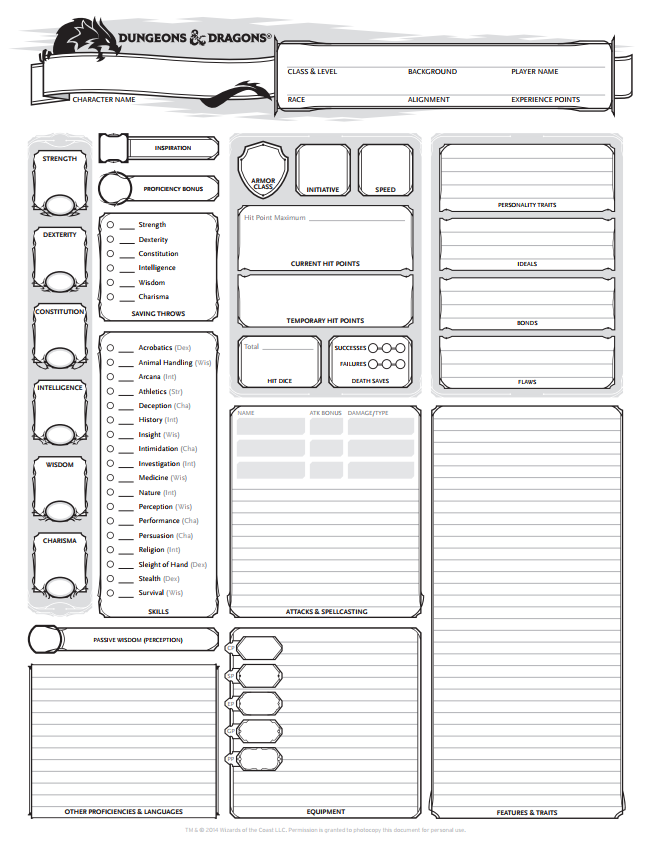
\includegraphics{character-sheet.png}
	\caption{D\&D5E Character Sheet}
	\label{fig:appa}
\end{figure}

\section{D\&D5E Spellcasting Sheet}
\begin{figure}
	\centering
	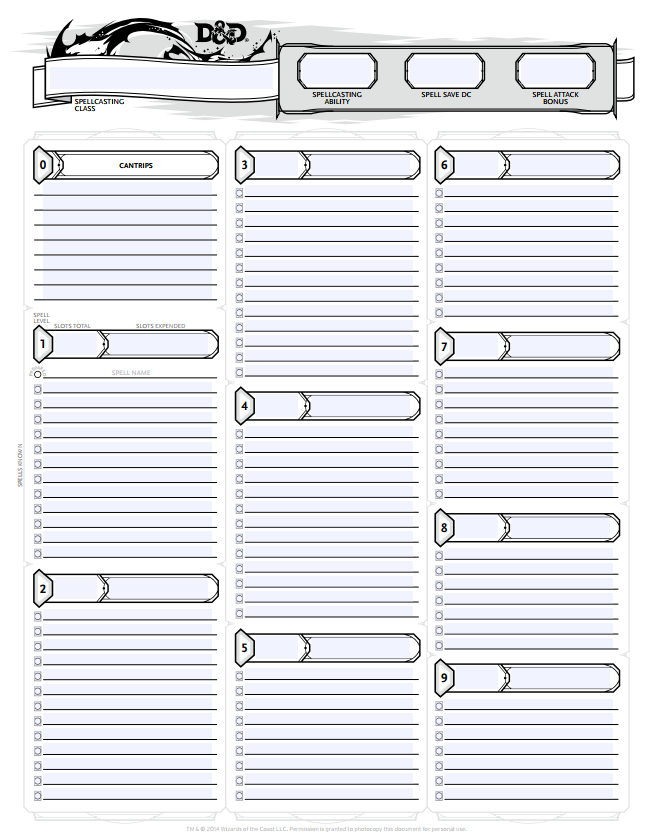
\includegraphics{spell-sheet}
	\caption{D\&D5E Spellcasting Sheet}
	\label{fig:appb}
\end{figure}

\end{document}
